\chapter{从边界条件到开弦谱}

\lectureoverview{我们的目标是量子化一根开弦，并判定它的态是否配得上被称为粒子。这条路线是初等的，但要求严格。我们首先准备 \(0\leq\sigma\leq\pi\) 上函数的微积分与傅里叶分析。随后，我们用粒子行为的谱判据取代点状性，回顾横向动力学变为非相对论性的无限动量描述，并用一链轻质量与刚性弹簧构造弦。连续弦是一个具有自由端点的波动系统。它的诺伊曼模解耦为频率为 \(1,2,3,\ldots\) 的谐振子；因此量子化产生离散的、有能隙的谱。弦的相互作用最终迫使我们超出开弦：一根开弦可以把自己的端点连接起来而变成闭弦。}

\section{开弦区间上的微积分}

计算将反复把离散求和变为积分，把最近邻差分变为导数。最好在它们打断物理讨论之前先把这些事实准备好。

设 \(x(\sigma)\) 是定义在

\begin{equation}
  0\leq \sigma\leq \pi .
\end{equation}

记号已经预示了弦论：\(\sigma\) 标记沿弦的位置，而 \(x\) 将成为它的一个横向坐标。把区间分成 \(N\) 段，

\begin{equation}
  \Delta\sigma=\frac{\pi}{N},
  \qquad
  \sigma_i=i\,\Delta\sigma,
  \qquad
  x_i=x(\sigma_i).
  \label{eq:l02-lattice}
\end{equation}

对于光滑的极限函数，

\begin{equation}
  \Delta x_i\equiv x_i-x_{i-1}
  =
  \frac{\partial x}{\partial\sigma}\,\Delta\sigma
  +O\!\left((\Delta\sigma)^2\right),
  \label{eq:l02-difference}
\end{equation}

而黎曼和变为

\begin{equation}
  \sum_i x_i\,\Delta\sigma
  \longrightarrow
  \int_0^\pi x(\sigma)\,d\sigma .
  \label{eq:l02-riemann}
\end{equation}

\begin{figure}[H]
  \centering
  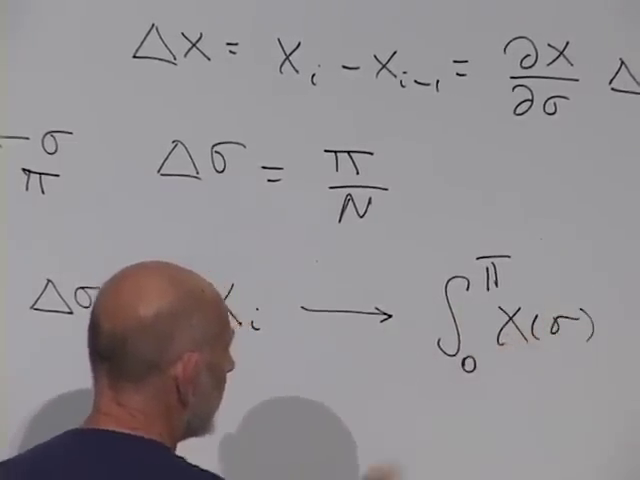
\includegraphics[width=0.78\textwidth]{lecture_02_figure_01.png}
  \caption{为后续连续极限保留在黑板上的有限差分与黎曼和规则。}
  \lectureframe{00:04:20}
  \label{fig:l02-calculus-board}
\end{figure}

这些都是微积分中熟悉的定义。它们在这里的重要性在于标度：\(\Delta x_i\) 带来一个 \(\Delta\sigma\) 的幂，而一个求和变为积分时则带来一个逆幂。

\subsection{狄利克雷端点与诺伊曼端点}

有限区间上的傅里叶分析始于端点处的一种选择。有两种选择会反复出现。

\begin{align}
  \text{Dirichlet:}\qquad
  &x(0)=x(\pi)=0,
  \label{eq:l02-dirichlet}\\
  \text{Neumann:}\qquad
  &\left.\partial_\sigma x\right|_{\sigma=0}
   =
   \left.\partial_\sigma x\right|_{\sigma=\pi}
   =0.
  \label{eq:l02-neumann}
\end{align}

两端被固定的提琴弦给出狄利克雷图像：其位移在边界处为零。诺伊曼函数则不必在边界处为零；它以零斜率与每个边界相接。这两种特征形状一起显示在黑板上。

\begin{figure}[H]
  \centering
  \begin{minipage}[t]{0.48\textwidth}
    \centering
    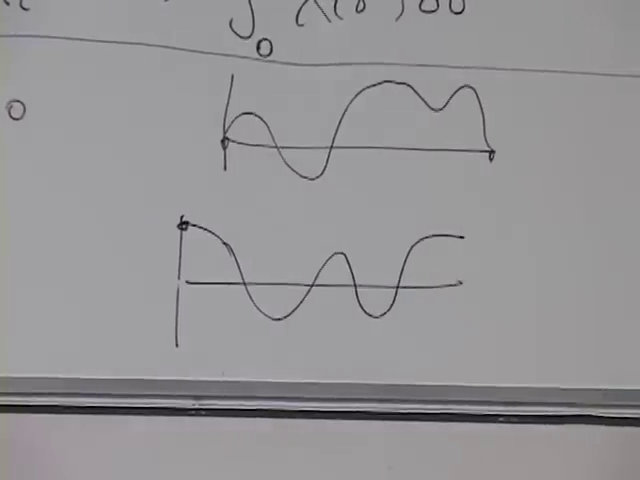
\includegraphics[width=\textwidth]{lecture_02_figure_02.png}
    \par\smallskip\footnotesize (a) 被钉住且平坦的端点剖面。
  \end{minipage}\hfill
  \begin{minipage}[t]{0.48\textwidth}
    \centering
    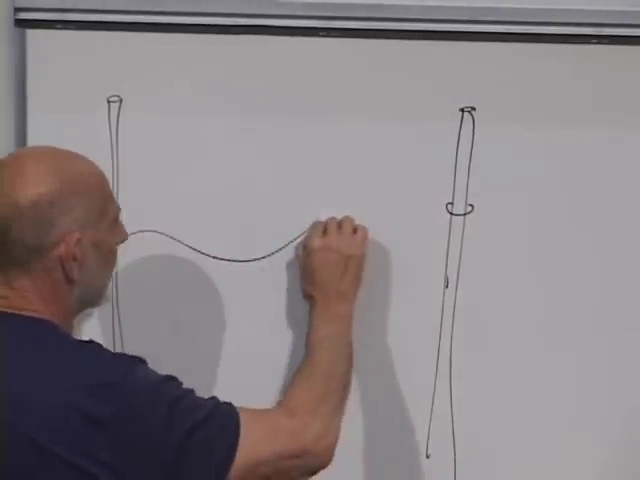
\includegraphics[width=\textwidth]{lecture_02_figure_03.png}
    \par\smallskip\footnotesize (b) 在竖直杆上滑动的轻环。
  \end{minipage}
  \caption{作为形状与力学的边界条件。滑动环构造赋予自由端点一个明确的横向运动。}
  \lectureframe{00:08:50 and 00:12:15}
  \label{fig:l02-boundaries-board}
\end{figure}

\begin{figure}[H]
  \centering
  \begin{adjustbox}{max width=\linewidth}
  \begin{tikzpicture}[>=Latex,thick,scale=0.92]
    \begin{scope}
      \draw[->] (0,0) -- (4.4,0) node[right] {\(\sigma\)};
      \draw[->] (0,-1.25) -- (0,1.35) node[above] {\(x\)};
      \draw[blue!70!black]
        (0,0) .. controls (0.8,1.1) and (1.4,1.0) .. (2.0,0)
        .. controls (2.7,-1.0) and (3.4,-0.8) .. (4.1,0);
      \fill (0,0) circle (0.06);
      \fill (4.1,0) circle (0.06);
      \node at (2.05,-1.65) {Dirichlet: \(x=0\)};
    \end{scope}
    \begin{scope}[xshift=5.8cm]
      \draw[->] (0,0) -- (4.4,0) node[right] {\(\sigma\)};
      \draw[->] (0,-1.25) -- (0,1.35) node[above] {\(x\)};
      \draw[orange!85!black]
        (0,0.65) .. controls (0.8,0.65) and (1.1,-0.9) .. (2.0,-0.9)
        .. controls (2.9,-0.9) and (3.2,0.55) .. (4.1,0.55);
      \draw[orange!85!black] (0,0.65) -- (0.45,0.65);
      \draw[orange!85!black] (3.65,0.55) -- (4.1,0.55);
      \node at (2.05,-1.65) {Neumann: \(\partial_\sigma x=0\)};
    \end{scope}
  \end{tikzpicture}
  \end{adjustbox}
  \caption{对于狄利克雷数据，函数值固定；对于诺伊曼数据，斜率固定。}
  \label{fig:l02-boundaries-redraw}
\end{figure}

\begin{classroomqa}
\audiencequestion{开管或闭管风琴能否为这些边界条件之一提供一个清晰的例子？\lecturetimestamp{00:09:19}}
\lecturerresponse{可以，但首先必须说明正在展开的是哪个声学变量。压力扰动与纵向位移在开口端服从互补的理想化条件。与其在黑板上解决这个枝节问题，不如使用滑动环模型：近乎无质量的环可以在杆上竖直移动，因此弦的端点是自由的，诺伊曼图像是直接的。}
\end{classroomqa}

\begin{classroomqa}
\audiencequestion{图像能否竖直上升并包含一个尖锐的跳跃？\lecturetimestamp{00:09:53}}
\lecturerresponse{傅里叶分析允许分段连续函数中存在孤立跳跃。物理弦则更具限制性。一个跳跃会断开相邻点，并使空间导数 \(\partial_\sigma x\) 在下面导出的连续能量中奇异。因此我们只关注连续且可微的剖面。}
\end{classroomqa}

\begin{classroomqa}
\audiencequestion{为什么管子的开口端，或任何自由端，竟然要满足边界条件？\lecturetimestamp{00:11:14}}
\lecturerresponse{声学例子取决于所选的场，在讨论中未得到解决。力学例子则不然。一个非常轻的环可以自由滑动，但仍然连接在最后一段弦上。我们将从牛顿定律推导它的条件，而不是假设它：有限的端点加速度迫使斜率消失。}
\end{classroomqa}

\subsection{傅里叶基}

一旦端点类别固定，相应的傅里叶基也就固定。在 \(0\leq\sigma\leq\pi\) 上，

\begin{align}
  x_D(\sigma)
  &=
  \sum_{n=1}^{\infty}x_n\sin(n\sigma),
  \label{eq:l02-dirichlet-series}\\
  x_N(\sigma)
  &=
  \sum_{n=0}^{\infty}x_n\cos(n\sigma).
  \label{eq:l02-neumann-series}
\end{align}

\eqref{eq:l02-dirichlet-series} 中的每个正弦都在两个端点处为零。
\eqref{eq:l02-neumann-series} 中的每个余弦都有零端点导数。
下限不同是有原因的：
\(\sin(0\sigma)=0\) 不贡献任何东西，而
\(\cos(0\sigma)=1\) 是常数模，或零模。它记录诺伊曼函数的平均值。

\begin{figure}[H]
  \centering
  \begin{minipage}[t]{0.48\textwidth}
    \centering
    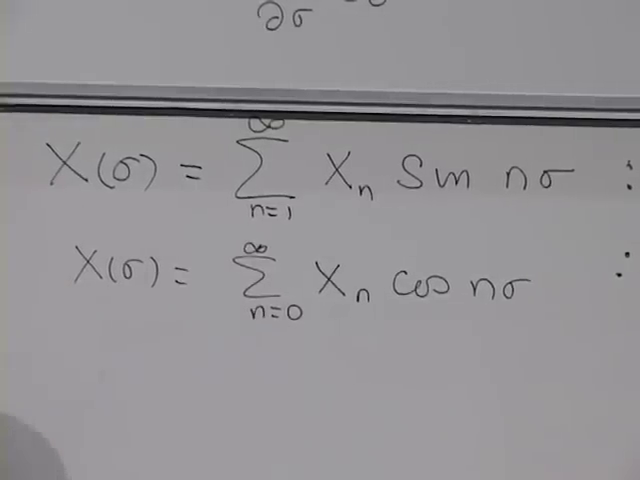
\includegraphics[width=\textwidth]{lecture_02_figure_04.png}
    \par\smallskip\footnotesize (a) 正弦与余弦展开。
  \end{minipage}\hfill
  \begin{minipage}[t]{0.48\textwidth}
    \centering
    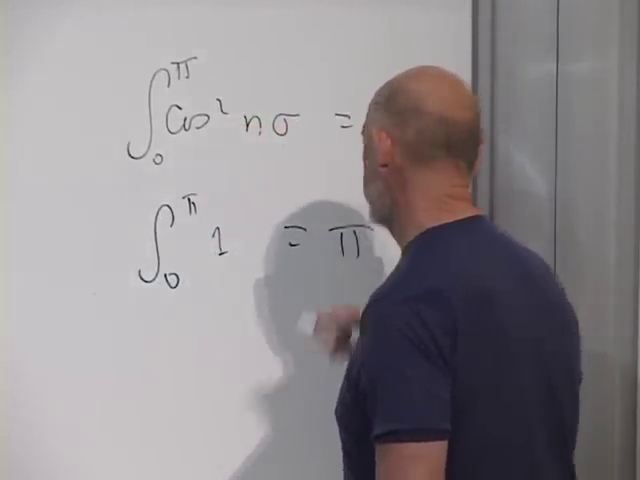
\includegraphics[width=\textwidth]{lecture_02_figure_05.png}
    \par\smallskip\footnotesize (b) 正交性与例外的
    常数模式。
  \end{minipage}
  \caption{后文用于将弦对角化的傅里叶事实。}
  \lectureframe{00:16:15 and 00:20:30}
  \label{fig:l02-fourier-board}
\end{figure}

求导交换这两类：

\begin{equation}
  \begin{aligned}
    \partial_\sigma\sin(n\sigma)&=n\cos(n\sigma),\\
    \partial_\sigma\cos(n\sigma)&=-n\sin(n\sigma).
  \end{aligned}
  \label{eq:l02-basis-derivatives}
\end{equation}

因此，Dirichlet 级数的导数具有 Neumann 行为，而 Neumann 级数的导数具有 Dirichlet 行为。正交性随后消去不同模式之间的交叉项：

\begin{align}
  \int_0^\pi\cos(n\sigma)\cos(m\sigma)\,d\sigma
  &=
  \frac{\pi}{2}\delta_{nm},
  && n,m\geq1,
  \label{eq:l02-cos-orthogonality}\\
  \int_0^\pi\sin(n\sigma)\sin(m\sigma)\,d\sigma
  &=
  \frac{\pi}{2}\delta_{nm},
  && n,m\geq1,
  \label{eq:l02-sin-orthogonality}\\
  \int_0^\pi 1\,d\sigma&=\pi .
  \label{eq:l02-zero-norm}
\end{align}

最后一行是例外的 \(n=m=0\) 余弦范数。常数并不像非零谐波那样被归一化，而那个因子二将把弦的质心模式与其内部模式区分开来。

\subsection{一个要记住的振子公式}

在重新标度坐标使其力学质量为 1 之后，胡克定律振子有

\begin{align}
  E_{\mathrm{osc}}
  &=
  \frac12\dot q^{\,2}
  +\frac12\omega^2q^2,
  \label{eq:l02-oscillator-energy}\\
  L_{\mathrm{osc}}
  &=
  \frac12\dot q^{\,2}
  -\frac12\omega^2q^2.
  \label{eq:l02-oscillator-lagrangian}
\end{align}

\begin{figure}[H]
  \centering
  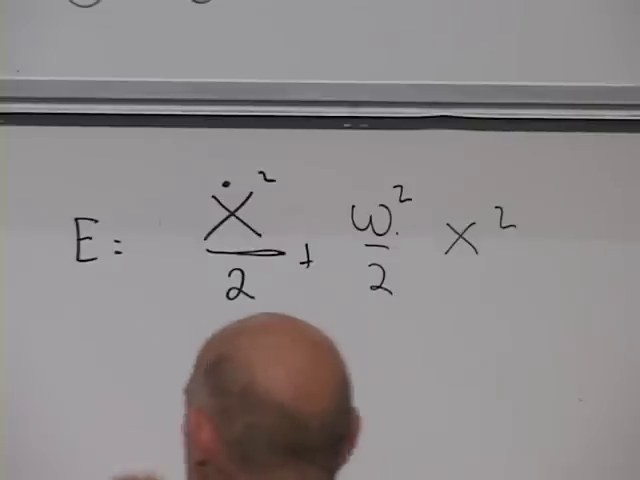
\includegraphics[width=0.68\textwidth]{lecture_02_figure_06.png}
  \caption{振子能量，如此写出使得 \(q^2\) 的系数
  立即标识出 \(\omega^2\)。}
  \lectureframe{00:24:00}
  \label{fig:l02-oscillator-board}
\end{figure}

经典地，\(\omega=\sqrt{\kappa/m}\)；坐标的重新标度已设定
\(m=1\)。量子力学地，

\begin{equation}
  E_Q=\hbar\omega\left(Q+\frac12\right),
  \qquad Q=0,1,2,\ldots .
  \label{eq:l02-oscillator-spectrum}
\end{equation}

对于能级间距，我们可以减去共同的基态项，并说每个量子花费 \(\hbar\omega\)。弦的计算最初将恰好这样做，并推迟总零点能。

\begin{classroomqa}
\audiencequestion{如何从能量公式读出振子频率？\lecturetimestamp{00:23:21}}
\lecturerresponse{在重新标度之前它是
\(\omega=\sqrt{\kappa/m}\)。在单位质量下，势项为
\(\frac12\omega^2q^2\)，因此其二次系数就是频率的平方。}
\end{classroomqa}

\section{是什么使一个复合系统成为粒子？}

弦是延展的，并将由许多耦合的片段来建模。那么，在什么意义上它的一个量子态仍可以是粒子？点状性不能是决定性的判据。质子和中子是复合的。电子和光子即使没有分辨出任何内禀子结构，也伴随着量子场的缀饰。一个周围空无一物的经典几何点并不是量子激发的正确图像。

质量和质心位置也不充分。一个密封的气体盒子两者都有。一杯咖啡两者都有。我们通常不把其中任何一个称为粒子。不可分性也不成立，因为质子是可分的，而自旋并不区分微观粒子与宏观物体。

有用的判据是谱隔离。把静能放在竖直轴上，并问需要多少能量才能到达另一个内部态。电子在紧邻其上方没有实验上可及的电子激发塔。质子确实有共振，但最初的几个共振要花费几百 MeV，即质子质量的相当一部分。那些态被分隔得足够开，可以逐个辨认。

一杯咖啡则相反。人们可以向一个长波长声模式加入任意小的能量，轻推一个分子，或产生一个声子。有极多的态挤在一个微小的间隔内。在实验室尺度上，它们形成一个连续统。这就是粒子与 \emph{糊状物} 之间的实际区别。

\begin{figure}[H]
  \centering
  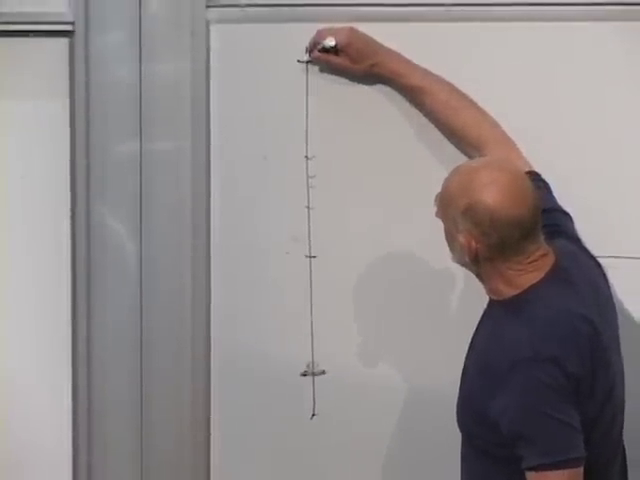
\includegraphics[width=0.58\textwidth]{lecture_02_figure_07.png}
  \caption{在比较孤立粒子能级与普通物质的密集激发时，黑板上的竖直能量轴。}
  \lectureframe{00:31:10}
  \label{fig:l02-spectrum-board}
\end{figure}

\begin{figure}[H]
  \centering
  \begin{adjustbox}{max width=\linewidth}
  \begin{tikzpicture}[>=Latex,thick]
    \begin{scope}
      \draw[->] (0,0) -- (0,4.8) node[above] {energy};
      \draw[blue!70!black,line width=1.2pt] (-1.0,0.65) -- (1.0,0.65);
      \draw[blue!70!black,line width=1.2pt] (-1.0,3.65) -- (1.0,3.65);
      \node[right] at (1.05,0.65) {ground state};
      \node[right] at (1.05,3.65) {first internal excitation};
      \draw[<->] (0.65,0.75) -- (0.65,3.55)
        node[midway,right] {large gap};
      \node at (0,-0.55) {particle-like};
    \end{scope}
    \begin{scope}[xshift=7.0cm]
      \draw[->] (0,0) -- (0,4.8) node[above] {energy};
      \foreach \y in {0.55,0.69,0.82,0.94,1.05,1.15,1.24,1.32,1.39,1.45,
        1.51,1.57,1.63,1.70,1.78,1.87,1.97,2.09,2.22,2.36,2.51,2.67,2.84,
        3.02,3.21,3.41,3.62,3.84,4.07}
        \draw[orange!85!black] (-0.95,\y) -- (0.95,\y);
      \node[right] at (1.05,2.25) {dense phonon and internal states};
      \node at (0,-0.55) {macroscopic matter};
    \end{scope}
  \end{tikzpicture}
  \end{adjustbox}
  \caption{谱隔离，而非字面上的点状性，是讲座中使用的操作性粒子判据。}
  \label{fig:l02-particle-redraw}
\end{figure}

这个判据把哲学问题变成了一个计算。量子化弦，找出它的内部能级，并检查它们的间距。如果弦的第一激发态位于普朗克尺度附近，而观测到的基态很轻，那么这个间隙超过当前加速器能量二十多个数量级。于是弦在整个可及范围内都表现为一个基本粒子。

\begin{classroomqa}
\audiencequestion{粒子行为仅仅是一个观测尺度的问题吗？如果我们放大得足够远，能级会不再分离吗？\lecturetimestamp{00:33:33}}
\lecturerresponse{放大可能揭示一个物体有许多组分，但并不会抹去谱。相关的比较是实验的能量分辨率与到第一内部激发的间隙之间的比较。当那个间隙巨大时，一个复合物体可以保持类粒子性。}
\end{classroomqa}

\begin{classroomqa}
\audiencequestion{为什么普通的小提琴弦不是粒子？\lecturetimestamp{00:34:37}}
\lecturerresponse{一个振动量子所携带的能量与宏观弦的静止能量相比小得无法测量。因此许多量子态都挤在一个极小的相对间隔内。它属于谱比较中密集的一侧，而不是孤立的一侧。}
\end{classroomqa}

\begin{classroomqa}
\audiencequestion{如果量子场以虚涨落环绕光子和电子，它们还是点粒子吗？\lecturetimestamp{00:35:40}}
\lecturerresponse{经典意义上的\emph{点}这个词承担了太多含义。物理上的电子和光子是着装场激发，然而实验尚未发现二者具有内禀组分结构或有限形状因子。对当前论证而言，重要的是二者都没有密集的近似简并内态塔。\editorialnote{讲座将电子的反常磁矩与可测量的量子模糊性联系起来。用现代术语来说，反常磁矩是一种辐射着装效应，而不是电子具有可分辨有限半径的证据。点状按惯例意味着在已检验的尺度上尚未探测到任何内禀子结构或形状因子。}}
\end{classroomqa}

\begin{classroomqa}
\audiencequestion{光子的大小取决于它的频率吗？\lecturetimestamp{00:36:49}}
\lecturerresponse{它的波长当然取决于频率。这与内禀组分大小不同。改变频率改变的是波包和波长，而不是光子可分辨的内部半径。}
\end{classroomqa}

\section{大动量下的精确横向力学}

现在我们回到相对论性困难。一根快速旋转的短棒不能仅仅通过把其质心置于静止就作非相对论处理。它的两端相对于彼此仍然作相对论性运动。非相对论近似之所以失效，是因为存在内部相对运动。

然而，存在另一种极限。选取一根\(z\)轴，将整个系统助推到非常大的正纵向动量\(P_z\)。保持其横向动量

\begin{equation}
  p_\perp^2=p_x^2+p_y^2
\end{equation}

有限。于是在\(P_z\to\infty\)极限下，横向投影允许一个精确的非相对论哈密顿量形式，即使未助推的内部运动是相对论性的。

\begin{classroomqa}
\audiencequestion{无限动量是否意味着有质量的系统实际达到了光速？\lecturetimestamp{00:40:43}}
\lecturerresponse{任何有限助推都达不到光速。人们构造的是当\(P_z\)变得任意大时具有良定义极限的量。这个说法命名的是一种取极限的程序，而不是一个具有\(v=c\)的有限物理状态。}
\end{classroomqa}

\begin{classroomqa}
\audiencequestion{必须选取哪根轴？如果物体绕该轴旋转或横穿该轴，又会怎样？\lecturetimestamp{00:41:14}}
\lecturerresponse{可以选取任意轴，并沿该轴助推整个系统。作为显式力学保留下来的，是到垂直平面上的投影。一根旋转的杆可能看起来被透视缩短，或扫过该平面，但它的横向投影具有非相对论形式。}
\end{classroomqa}

弦还有一个额外性质，使这种表示异常强大。在光前规范中，它们的纵向内部坐标不是独立振子。约束由横向运动决定它们。因此，知道横向弦就足以重构物理自由度。

\begin{classroomqa}
\audiencequestion{不存在独立的纵向坐标，是否意味着弦只是被困在一个薄三明治中？\lecturetimestamp{00:42:26}}
\lecturerresponse{洛伦兹收缩确实使它在助推系中的纵向延展变小，但这个陈述更强。任何残余的纵向运动都受到横向运动的约束；它不能被独立指定。}
\end{classroomqa}

\begin{classroomqa}
\audiencequestion{这种向横向数据的约化与全息原理有关吗？\lecturetimestamp{00:43:12}}
\lecturerresponse{它与导致全息思想的那条思路密切相关，不过追究这一联系会使我们偏离当前的计算。在这里，它只用于证明使用横向弦是合理的。}
\end{classroomqa}

\subsection{减去助推并重新标度时间}

设\(M\)为整个系统的不变质量，包括组分质量、动能和束缚能。在单位\(c=1\)下，

\begin{equation}
  E=\sqrt{P_z^2+p_\perp^2+M^2}.
  \label{eq:l02-relativistic-energy}
\end{equation}

当\(P_z\)远大于\(p_\perp\)和\(M\)时，

\begin{equation}
  E
  =
  P_z+\frac{p_\perp^2+M^2}{2P_z}
  +O(P_z^{-3}).
  \label{eq:l02-large-pz}
\end{equation}

\begin{figure}[H]
  \centering
  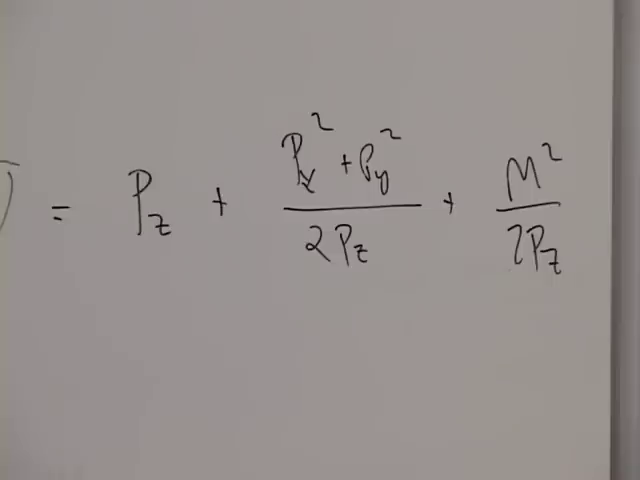
\includegraphics[width=0.76\textwidth]{lecture_02_figure_08.png}
  \caption{完成的大\(P_z\)展开，其中保留了横向动量和不变质量。}
  \lectureframe{00:47:30}
  \label{fig:l02-large-pz-board}
\end{figure}

领头项很大，但它不携带任何关于内部状态的信息。在守恒\(P_z\)的过程中，例如一个被加速的原子在不改变其总纵向动量的情况下于内部能级之间跃迁，该项会从每个能量差中消去。因此我们研究

\begin{equation}
  E-P_z=\frac{p_\perp^2+M^2}{2P_z}+O(P_z^{-3}).
  \label{eq:l02-residual-energy}
\end{equation}

分母具有物理意义。由于哈密顿量生成时间演化，这个小的剩余能量表明内部演化在实验室时间中显得缓慢。这就是时间膨胀。为了保留内部运动，引入一个重新标度的演化参数\(\tau\)，或者等价地将剩余哈密顿量乘以\(P_z\)：

\begin{equation}
  H_\perp
  \equiv
  \lim_{P_z\to\infty}P_z(E-P_z)
  =
  \frac12p_\perp^2+\frac12M^2.
  \label{eq:l02-transverse-hamiltonian}
\end{equation}

\begin{figure}[H]
  \centering
  \begin{minipage}[t]{0.48\textwidth}
    \centering
    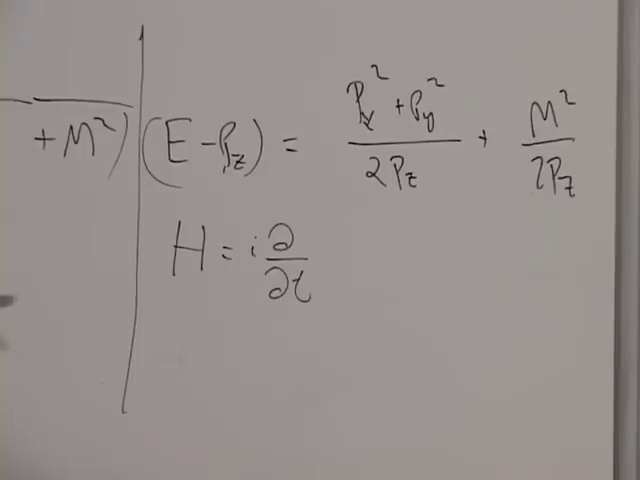
\includegraphics[width=\textwidth]{lecture_02_figure_09.png}
    \par\smallskip\footnotesize (a) \(H=i\partial_t\) 以及被减慢的内部
    演化。
  \end{minipage}\hfill
  \begin{minipage}[t]{0.48\textwidth}
    \centering
    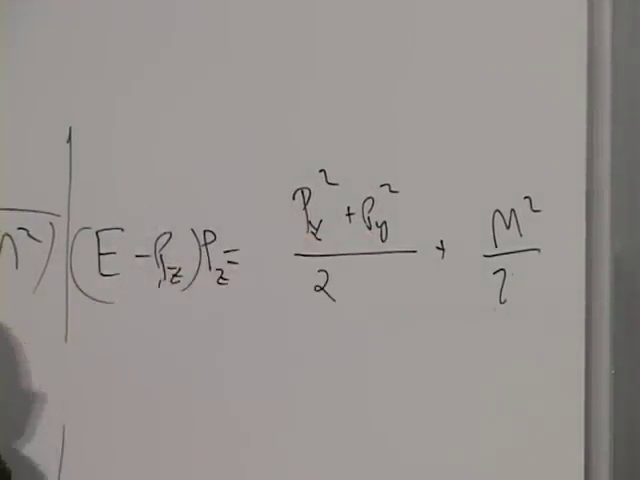
\includegraphics[width=\textwidth]{lecture_02_figure_10.png}
    \par\smallskip\footnotesize (b) 时间重标度之后的有限横向哈密顿量。
  \end{minipage}
  \caption{从时间膨胀的剩余能量到有限的
  二维哈密顿量。}
  \lectureframe{00:49:20 and 00:52:40}
  \label{fig:l02-lightfront-board}
\end{figure}

这正是一个单位质量粒子在二维中运动的哈密顿量形式：动能\(p_\perp^2/2\)加上内部能量\(M^2/2\)。不寻常的特征在于平方。在这一描述中，扮演静止能量或束缚能量角色的量正比于不变质量的平方。\editorialnote{采用传统的光前变量\(P^\pm=(E\pm P_z)/\sqrt2\)时，精确的质壳关系为\(2P^+P^-=p_\perp^2+M^2\)。方程\eqref{eq:l02-transverse-hamiltonian}是本讲中同一不变关系的大\(P_z\)归一化形式。}

\begin{classroomqa}
\audiencequestion{复合系统各个组成部分的纵向动量到哪里去了？\lecturetimestamp{00:51:30}}
\lecturerresponse{对于一般的复合客体，必须保留其组分所携带的总\(P_z\)的分数。上面的公式使用了总质心动量。弦理论之所以特殊，是因为其约束从横向自由度决定了相对纵向运动，因此不需要添加独立的纵向振子。}
\end{classroomqa}

\section{离散开弦}

被加速的弦现在明确地只在横向平面中运动。将其两个坐标标记为\(X\)和\(Y\)，并首先用\(N\)个质点由\(N-1\)根弹簧连接来近似它。如果\(\mu\)是每个质点的类比质量，\(k\)是最近邻弹簧常数，则能量为

\begin{equation}
  E_N
  =
  \sum_i
  \left[
    \frac{\mu}{2}
    \left(\dot X_i^2+\dot Y_i^2\right)
    +
    \frac{k}{2}
    \left((\Delta X_i)^2+(\Delta Y_i)^2\right)
  \right].
  \label{eq:l02-discrete-energy}
\end{equation}

每个\(X\)项都有一个相同的\(Y\)项，因为横向平面有两个方向。指标\(i\)标记链上的一个点；它不是空间坐标。

\begin{figure}[H]
  \centering
  \begin{minipage}[t]{0.48\textwidth}
    \centering
    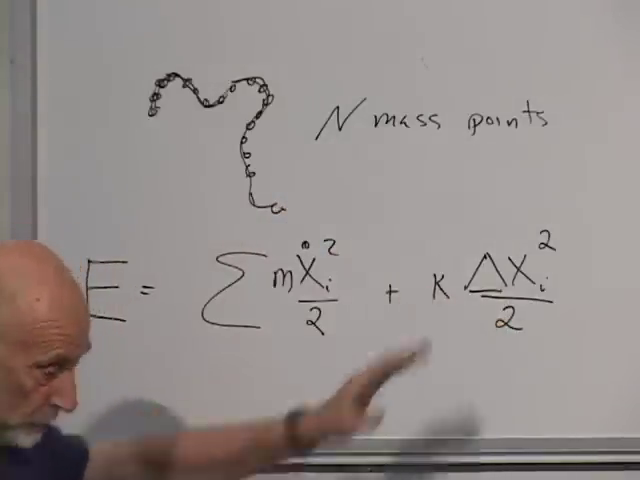
\includegraphics[width=\textwidth]{lecture_02_figure_11.png}
    \par\smallskip\footnotesize (a) 珠链及其离散能量。
  \end{minipage}\hfill
  \begin{minipage}[t]{0.48\textwidth}
    \centering
    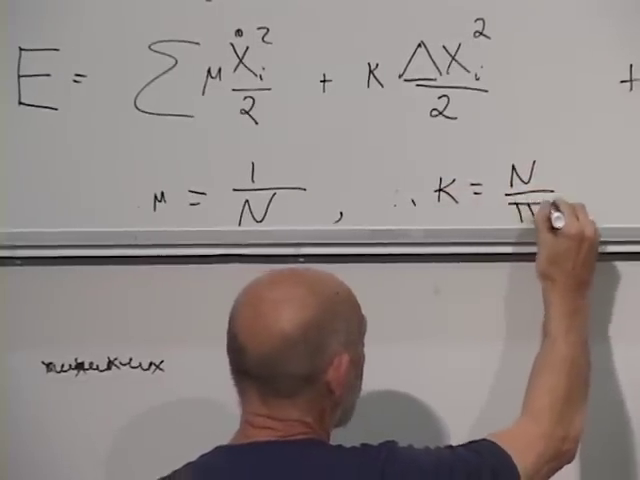
\includegraphics[width=\textwidth]{lecture_02_figure_12.png}
    \par\smallskip\footnotesize (b) \(\mu\)和\(k\)的大\(N\)标度行为。
  \end{minipage}
  \caption{取连续极限之前的正则化开弦。}
  \lectureframe{00:57:42 and 01:02:40}
  \label{fig:l02-chain-board}
\end{figure}

\begin{figure}[H]
  \centering
  \begin{adjustbox}{max width=\linewidth}
  \begin{tikzpicture}[>=Latex,thick]
    \foreach \i in {0,...,8} {
      \coordinate (p\i) at ({1.05*\i},{0.30*sin(55*\i)});
      \filldraw[white] (p\i) circle (0.10);
      \draw (p\i) circle (0.10);
    }
    \foreach \i in {0,...,7} {
      \pgfmathtruncatemacro{\j}{\i+1}
      \draw[decorate,decoration={zigzag,segment length=4pt,amplitude=2pt}]
        (p\i) -- (p\j);
    }
    \node[above=0.35cm of p0] {\(i=0\)};
    \node[above=0.35cm of p8] {\(i=N-1\)};
    \draw[<->] (0,-1.15) -- (8.4,-1.15)
      node[midway,below] {\(0\leq\sigma\leq\pi\)};
    \node at (4.2,1.25)
      {\(\mu=1/N,\quad k=N/\pi^2,\quad\Delta\sigma=\pi/N\)};
  \end{tikzpicture}
  \end{adjustbox}
  \caption{一幅清晰的正则化图像。随着链被细化，质点变得更轻，而微观弹簧变得更硬。}
  \label{fig:l02-chain-redraw}
\end{figure}

参数\(\sigma\)标记沿链的位置。选择\(0\leq\sigma\leq\pi\)是一种约定，而不是物理长度测量。它提醒我们弦有两个端点。稍后闭弦将在\(0\leq\sigma<2\pi\)上周期性地标记。

连续极限必须保持集体力学量有限。固定的珠质量会使总类比质量发散，因此选择

\begin{equation}
  \mu=\frac{1}{N}.
  \label{eq:l02-mu-scaling}
\end{equation}

于是\(N\mu=1\)。这不是相对论静止质量\(M\)；它是横向类比模型中的惯性系数。

串联的弹簧随着数目增加而变软。为了使整条链保持有限的劲度，每根微观弹簧必须变得更硬：

\begin{equation}
  k=\frac{N}{\pi^2}
  =\frac{1}{\pi\,\Delta\sigma}.
  \label{eq:l02-k-scaling}
\end{equation}

只有\(k\propto N\)是本质的。因子\(\pi^2\)是为了从连续公式中消除多余的\(\pi\)因子而选择的归一化。

\begin{classroomqa}
\audiencequestion{\(\mu\)是每个弦点的物理静止质量吗？\lecturetimestamp{01:10:34}}
\lecturerresponse{不是。它是横向链中出现的非相对论类比质量。把它称为\(M\)会与整个相对论弦状态的不变静止质量相混淆。它目前唯一的作用是产生正确的连续惯性。}
\end{classroomqa}

\section{连续波系统}

应用开头准备好的规则。由于\(1/N=\Delta\sigma/\pi\)，

\begin{align}
  \sum_i\frac{\mu}{2}\dot X_i^2
  &=
  \frac{1}{2\pi}
  \sum_i\dot X_i^2\,\Delta\sigma
  \longrightarrow
  \frac{1}{2\pi}
  \int_0^\pi
  \left(\partial_\tau X\right)^2d\sigma ,
  \label{eq:l02-kinetic-limit}\\
  \sum_i\frac{k}{2}(\Delta X_i)^2
  &\longrightarrow
  \frac{1}{2\pi}
  \int_0^\pi
  \left(\partial_\sigma X\right)^2d\sigma .
  \label{eq:l02-potential-limit}
\end{align}

对于第二行，使用\(\Delta X_i=\partial_\sigma X\,\Delta\sigma\)以及\(k=1/(\pi\Delta\sigma)\)。同样的计算适用于\(Y\)。

\begin{figure}[H]
  \centering
  \begin{minipage}[t]{0.48\textwidth}
    \centering
    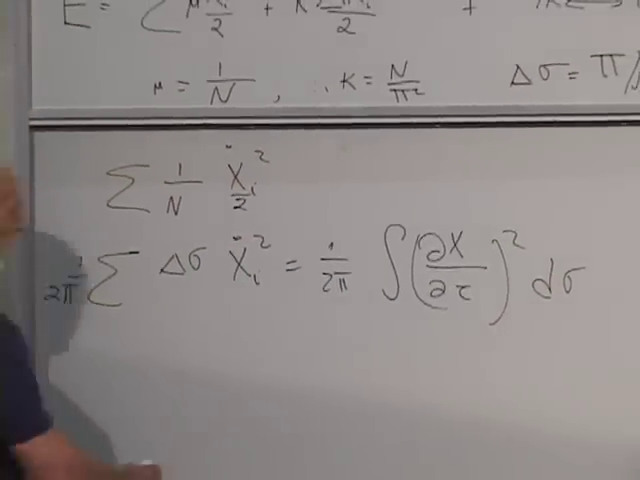
\includegraphics[width=\textwidth]{lecture_02_figure_13.png}
    \par\smallskip\footnotesize (a) 求和化为积分以及
    差分化为导数的替换。
  \end{minipage}\hfill
  \begin{minipage}[t]{0.48\textwidth}
    \centering
    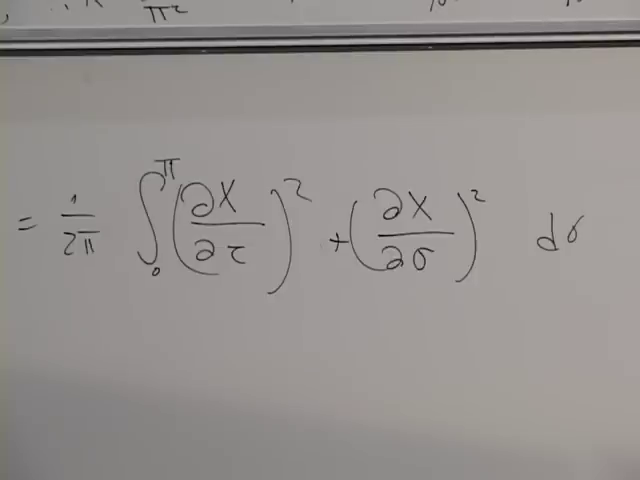
\includegraphics[width=\textwidth]{lecture_02_figure_14.png}
    \par\smallskip\footnotesize (b) 完成后的连续极限能量。
  \end{minipage}
  \caption{离散链在 \(\sigma\) 区间上变为场。}
  \lectureframe{01:05:40 and 01:07:00}
  \label{fig:l02-continuum-board}
\end{figure}

由此得到的能量和拉格朗日量为

\begin{align}
  E
  &=
  \frac{1}{2\pi}
  \int_0^\pi d\sigma\,
  \left[
    (\partial_\tau X)^2+(\partial_\tau Y)^2\right.\notag\\[-0.25em]
  &\hspace{6.5em}\left.
    +(\partial_\sigma X)^2+(\partial_\sigma Y)^2
  \right],
  \label{eq:l02-continuum-energy}\\
  L
  &=
  \frac{1}{2\pi}
  \int_0^\pi d\sigma\,
  \left[
    (\partial_\tau X)^2+(\partial_\tau Y)^2\right.\notag\\[-0.25em]
  &\hspace{6.5em}\left.
    -(\partial_\sigma X)^2-(\partial_\sigma Y)^2
  \right].
  \label{eq:l02-continuum-lagrangian}
\end{align}

\begin{figure}[H]
  \centering
  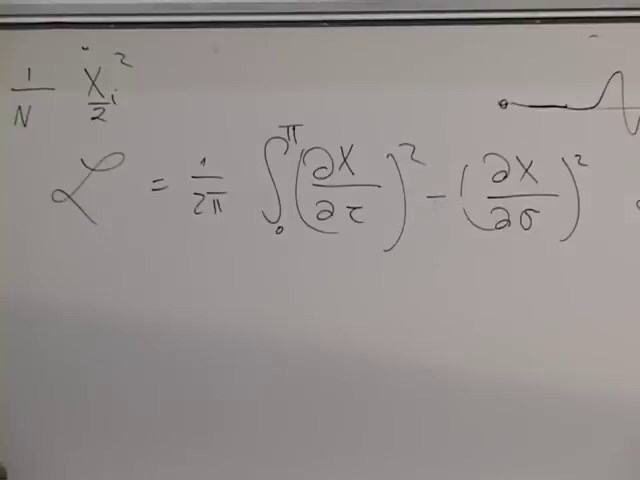
\includegraphics[width=0.78\textwidth]{lecture_02_figure_15.png}
  \caption{连续极限下的拉格朗日量，其动能项与拉伸项
  带有相反的符号。}
  \lectureframe{01:08:48}
  \label{fig:l02-lagrangian-board}
\end{figure}

如果我们把 \(\sigma\) 重新命名为一个普通空间坐标，把 \(X\) 重新命名为
一个场 \(\phi\)，那么这些就是一个一维波场的能量和拉格朗日量。对 \eqref{eq:l02-continuum-lagrangian} 作变分得到

\begin{equation}
  \left(\partial_\tau^2-\partial_\sigma^2\right)X=0,
  \qquad
  \left(\partial_\tau^2-\partial_\sigma^2\right)Y=0.
  \label{eq:l02-wave-equation}
\end{equation}

眼前的论证并不要求我们直接求解这些方程。有用的图像仅仅是：波沿弦向左和向右传播，并在端点处反射。Dirichlet 反射使位移改变符号；Neumann 反射则保持其符号不变。

\begin{classroomqa}
\audiencequestion{时间变量 \(\tau\) 究竟是什么？\lecturetimestamp{01:08:54}}
\lecturerresponse{它是在大 \(P_z\) 描述中用来追踪内部运动的重新标度时间。随系统一起作洛伦兹加速的时钟相对于实验室时间走得慢；\(\tau\) 消除了这种时间膨胀，使内部振荡保持有限的频率。对于这一横向力学而言，它可以简单地被当作时间来对待。\editorialnote{讲义中非正式地把 \(\tau\) 称为固有时。对于一根延展的弦，精确的光前演化参数是一个规范固定的重新标度时间，而不是每个点所共有的单一不变固有时。原本想要表达的时间膨胀论证并未改变。}}
\end{classroomqa}

当质心在横向平面内静止时，\eqref{eq:l02-continuum-energy} 的内部部分在
\eqref{eq:l02-transverse-hamiltonian} 的归一化下正比于 \(M^2\)。这就是为什么量子化这个表面上普通的波动系统会揭示出相对论性质量谱。

\begin{classroomqa}
\audiencequestion{\(P_z(E-P_z)\) 有
名称吗？\lecturetimestamp{01:11:00}}
\lecturerresponse{它通常被称为光锥能量或光前能量。
光前更好地描述了用作演化曲面的零平面；
传统术语对计算并不重要。}
\end{classroomqa}

\begin{classroomqa}
\audiencequestion{锥这个词是指通常的时空光锥吗，这个术语是 Dirac 引入的吗？\lecturetimestamp{01:11:17}}
\lecturerresponse{零坐标构造可以用
45 度轴来画出，但这里的演化曲面是一个光前，而不是完整的膨胀锥。Dirac 发展了相对论动力学的相关形式；历史命名问题仍悬而未决，且不影响方程。}
\end{classroomqa}

\section{为什么自由端点对应 Neumann}

我们现在可以推导而不是假设端点条件。牛顿定律是合法的，因为加速后的横向力学恰好具有非相对论形式。内部质点受到两侧弹簧的拉拽。最后一个点只受到将它与其相邻点连接起来的弹簧的拉拽。

\begin{classroomqa}
\audiencequestion{为什么在讨论相对论性弦时我们可以使用牛顿定律？\lecturetimestamp{01:14:52}}
\lecturerresponse{我们并不是把牛顿力学应用于完整的未加速时空运动。我们把它应用于无限动量描述中的横向变量，其哈密顿量恰好具有非相对论形式。}
\end{classroomqa}

在右端点处，胡克定律给出（不计取向）

\begin{equation}
  F_{\mathrm{end}}
  =
  -k\,\Delta X
  =
  -\frac{1}{\pi\Delta\sigma}
   \left(\partial_\sigma X\,\Delta\sigma\right)
  =
  -\frac{1}{\pi}\partial_\sigma X .
  \label{eq:l02-endpoint-force}
\end{equation}

\begin{figure}[H]
  \centering
  \begin{minipage}[t]{0.48\textwidth}
    \centering
    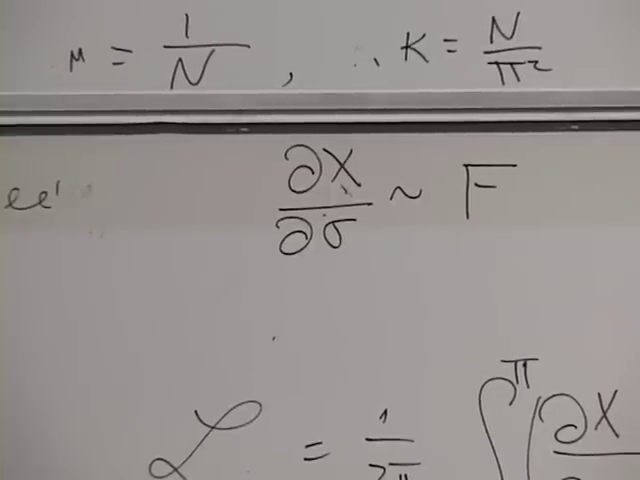
\includegraphics[width=\textwidth]{lecture_02_figure_16.png}
    \par\smallskip\footnotesize (a) 端点力正比于局部
    斜率。
  \end{minipage}\hfill
  \begin{minipage}[t]{0.48\textwidth}
    \centering
    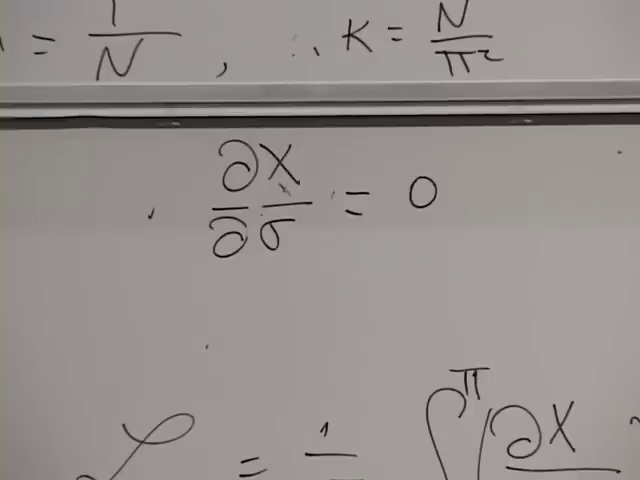
\includegraphics[width=\textwidth]{lecture_02_figure_17.png}
    \par\smallskip\footnotesize (b) 有限加速度条件。
  \end{minipage}
  \caption{自由端边界条件的牛顿定律推导。}
  \lectureframe{01:18:20 and 01:20:10}
  \label{fig:l02-neumann-board}
\end{figure}

最后一个点的牛顿方程为

\begin{equation}
  \mu\,\partial_\tau^2X=F_{\mathrm{end}},
  \qquad
  \mu=\frac1N=\frac{\Delta\sigma}{\pi}.
  \label{eq:l02-endpoint-newton}
\end{equation}

结合 \eqref{eq:l02-endpoint-force} 与
\eqref{eq:l02-endpoint-newton}，

\begin{equation}
  \partial_\sigma X
  =
  -\Delta\sigma\,\partial_\tau^2X
  \quad\text{at the right endpoint},
  \label{eq:l02-endpoint-scaling}
\end{equation}

在左端点处力的符号相反。如果
\(\partial_\sigma X\) 在
\(\Delta\sigma\to0\) 时趋于一个非零常数，则端点加速度将像 \(N\) 那样发散。
因此，一个具有有限加速度的合理连续极限要求

\begin{equation}
  \left.\partial_\sigma X\right|_{0,\pi}=0,
  \qquad
  \left.\partial_\sigma Y\right|_{0,\pi}=0.
  \label{eq:l02-open-neumann}
\end{equation}

\begin{figure}[H]
  \centering
  \begin{adjustbox}{max width=\linewidth}
  \begin{tikzpicture}[>=Latex,thick,scale=1.0]
    \coordinate (a) at (0,0);
    \coordinate (b) at (4.5,0.75);
    \filldraw[white] (a) circle (0.12);
    \draw (a) circle (0.12);
    \filldraw[white] (b) circle (0.12);
    \draw (b) circle (0.12);
    \draw[decorate,decoration={zigzag,segment length=6pt,amplitude=3pt}]
      (a) -- (b);
    \draw[dashed] (a) -- (0,-1.2);
    \draw[dashed] (b) -- (4.5,-1.2);
    \draw[<->] (4.85,0) -- (4.85,0.75)
      node[midway,right] {\(\Delta X\)};
    \draw[->,red!70!black] (b) -- (5.75,0.95)
      node[right] {\(F_{\rm end}=-k\Delta X\)};
    \node[below] at (0,-1.2) {\(N-1\)};
    \node[below] at (4.5,-1.2) {\(N\)};
    \node at (2.5,-2.0)
      {\(\mu\ddot X=-k\Delta X
      \ \Longrightarrow\
      \partial_\sigma X=-\Delta\sigma\,\ddot X\to0\)};
  \end{tikzpicture}
  \end{adjustbox}
  \caption{在正规化极限下最后一个点的质量趋于零。只有当端点斜率消失时，
  才可能有有限的加速度。}
  \label{fig:l02-neumann-redraw}
\end{figure}

在两端以及在两个横向方向上作同样的论证，就得到自由开弦的 Neumann 边界条件。

\section{开弦的简正模}

现在我们已经有了一个完整的经典系统：一个拉格朗日量及其边界条件。经过傅里叶分析之后，量子化就变得简单了。由于端点是诺伊曼端点，

\begin{align}
  X(\sigma,\tau)
  &=
  \sum_{n=0}^{\infty}X_n(\tau)\cos(n\sigma),
  \label{eq:l02-X-expansion}\\
  Y(\sigma,\tau)
  &=
  \sum_{n=0}^{\infty}Y_n(\tau)\cos(n\sigma).
  \label{eq:l02-Y-expansion}
\end{align}

余弦项包含了全部\(\sigma\)依赖。系数包含了全部时间依赖；弦之所以振动，是因为\(X_n(\tau)\)和\(Y_n(\tau)\)在变化。

\begin{figure}[H]
  \centering
  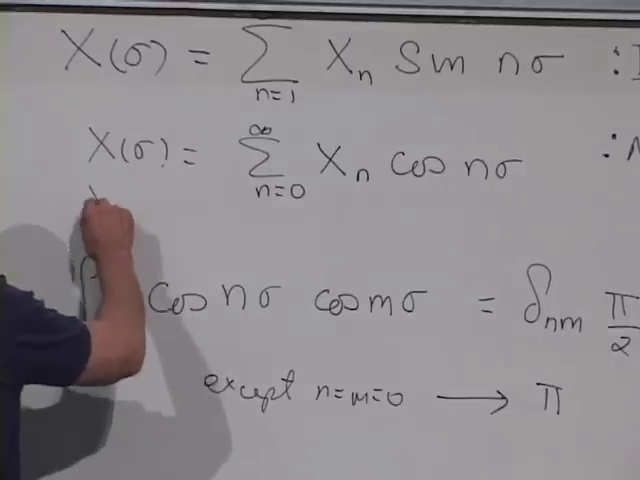
\includegraphics[width=0.78\textwidth]{lecture_02_figure_18.png}
  \caption{诺伊曼模展开式，与将把双重求和消去的正交性规则并列展示。}
  \lectureframe{01:21:45}
  \label{fig:l02-mode-expansion-board}
\end{figure}

\subsection{动能项与零模}

对时间求导给出

\begin{equation}
  \partial_\tau X
  =
  \sum_{n=0}^{\infty}\dot X_n(\tau)\cos(n\sigma).
  \label{eq:l02-time-mode}
\end{equation}

平方之后产生一个关于\(n\)和\(m\)的双重求和，但\eqref{eq:l02-cos-orthogonality}会消去每一个满足\(n\neq m\)的项。将常数模单独处理，

\begin{equation}
  \frac{1}{2\pi}\int_0^\pi
  (\partial_\tau X)^2\,d\sigma
  =
  \frac12\dot X_0^{\,2}
  +
  \frac14\sum_{n=1}^{\infty}\dot X_n^{\,2}.
  \label{eq:l02-mode-kinetic}
\end{equation}

\begin{figure}[H]
  \centering
  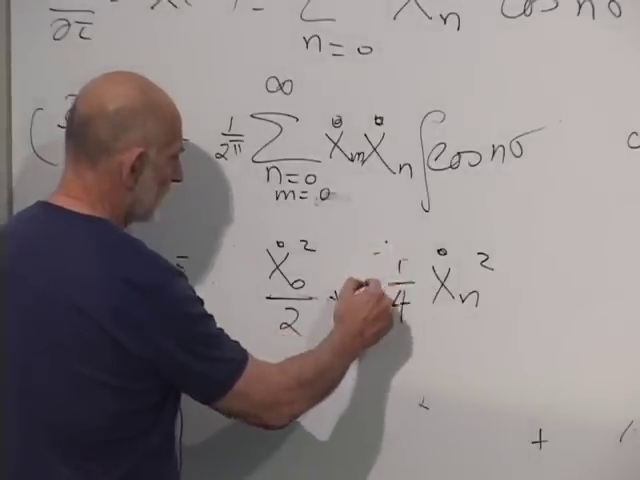
\includegraphics[width=0.76\textwidth]{lecture_02_figure_19.png}
  \caption{正交性积分将动能双重求和化为零模加上一个对角求和。}
  \lectureframe{01:29:10}
  \label{fig:l02-mode-kinetic-board}
\end{figure}

常数系数就是平均位置，

\begin{equation}
  X_0(\tau)=\frac1\pi\int_0^\pi X(\sigma,\tau)\,d\sigma ,
  \label{eq:l02-center-of-mass}
\end{equation}

对\(Y_0\)也类似。在均匀的模拟质量密度下，这些就是质心坐标。它们具有动能但没有回复力：整条弦可以在横向平面内自由运动。

\subsection{拉伸项与振子频率}

对空间求导给出

\begin{equation}
  \partial_\sigma X
  =
  -\sum_{n=1}^{\infty}nX_n(\tau)\sin(n\sigma).
  \label{eq:l02-spatial-mode}
\end{equation}

零模消失了，因为均匀平移不会拉伸弦。利用正弦正交性，

\begin{equation}
  \frac{1}{2\pi}\int_0^\pi
  (\partial_\sigma X)^2\,d\sigma
  =
  \frac14\sum_{n=1}^{\infty}n^2X_n^{\,2}.
  \label{eq:l02-mode-potential}
\end{equation}

\begin{figure}[H]
  \centering
  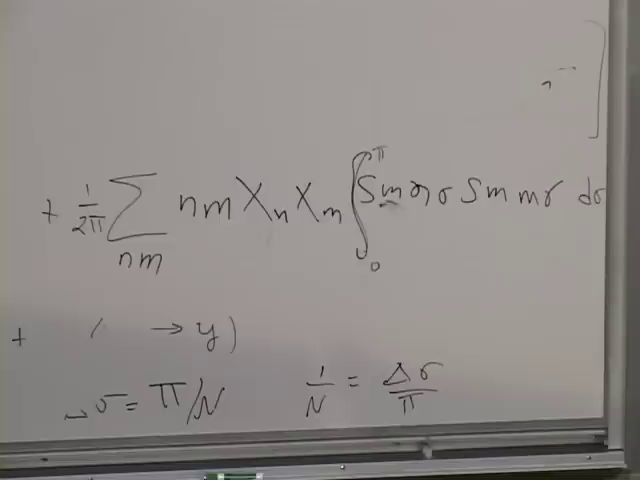
\includegraphics[width=0.76\textwidth]{lecture_02_figure_20.png}
  \caption{对余弦级数求导产生正弦双重求和；正交性再次强制\(n=m\)。}
  \lectureframe{01:31:40}
  \label{fig:l02-mode-potential-board}
\end{figure}

因此\(X\)部分的拉格朗日量为

\begin{equation}
  L_X
  =
  \frac12\dot X_0^{\,2}
  +
  \frac14\sum_{n=1}^{\infty}
  \left(
    \dot X_n^{\,2}-n^2X_n^{\,2}
  \right),
  \label{eq:l02-X-lagrangian}
\end{equation}

对\(Y\)有完全相同的表达式。相应的能量在\(n^2X_n^2\)前面有一个正号。每一个非零模都是一个独立的谐振子，与\eqref{eq:l02-oscillator-lagrangian}比较可得

\begin{equation}
  \omega_n=n,
  \qquad n=1,2,3,\ldots .
  \label{eq:l02-mode-frequency}
\end{equation}

\begin{figure}[H]
  \centering
  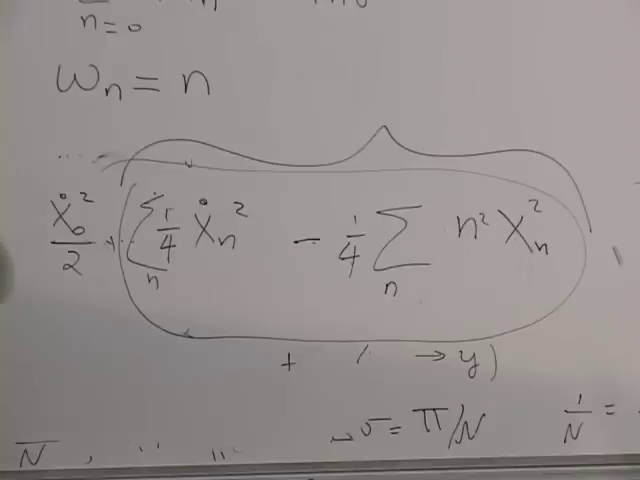
\includegraphics[width=0.80\textwidth]{lecture_02_figure_21.png}
  \caption{解耦的振子拉格朗日量以及结论\(\omega_n=n\)，下面还给出了完全相同的\(Y\)塔。}
  \lectureframe{01:35:50}
  \label{fig:l02-oscillator-modes-board}
\end{figure}

简正模就是弦的各个谐波。第一个缓慢弯曲，第二个频率是它的两倍，第三个是三倍，依此类推。正交性正是自由理论中防止一个谐波与另一个谐波耦合的原因。

\begin{classroomqa}
\audiencequestion{\(n=0\)振子怎么样了？\lecturetimestamp{01:34:49}}
\lecturerresponse{它的频率为零，因为它根本不是一个内部振子。它平移的是质心。没有任何弹簧会把整条弦恢复到某个偏好的横向位置，所以零模是一个自由粒子坐标。}
\end{classroomqa}

去掉质心动能项后，剩下的就是内能

\begin{equation}
  E_{\mathrm{int}}
  =
  \frac14
  \sum_{n=1}^{\infty}
  \left[
    \dot X_n^{\,2}+n^2X_n^{\,2}
    +\dot Y_n^{\,2}+n^2Y_n^{\,2}
  \right].
  \label{eq:l02-internal-energy}
\end{equation}

在光前归一化中，这正比于弦态的不变质量平方。这样我们就将相对论性质量问题转化成了两个可数振子塔的量子力学。

\section{量子化能级与粒子行为}

设\(a_n^\dagger\)在频率为\(n\)的\(X\)振子中产生一个量子，而\(b_n^\dagger\)对\(Y\)做同样的事。本讲推迟了系统的算符处理，但这种记号使能级计数变得透明。相对于基态偏移，

\begin{equation}
  \begin{aligned}
    \Delta E_{\mathrm{int}}
    &=\sum_{n=1}^{\infty}n\left(Q_n^X+Q_n^Y\right),\\
    Q_n^X,Q_n^Y&\in\{0,1,2,\ldots\}.
  \end{aligned}
  \label{eq:l02-quantized-energy}
\end{equation}

其中\(\hbar=1\)。整数\(n\)标记哪个振子被激发；\(Q_n\)计算它占据了多少个量子。\editorialnote{每个振子还贡献一份零点能。这个无穷求和需要正规化，并提供了弦质量公式的截距。本讲在此有意不指定基态偏移，只计激发能级。}

振子真空\(\ket{0}\)并不是空无一物的时空。它是一条没有内部振子被激发的开弦。它具有能量、动量，并在弦谱中占有确定的位置。

在第一能级上有两个态，

\begin{equation}
  a_1^\dagger\ket{0},
  \qquad
  b_1^\dagger\ket{0},
  \label{eq:l02-level-one}
\end{equation}

对应于沿\(X\)或\(Y\)极化的最低谐波。线性组合描述任意横向极化。

在第二能级上有五个态：

\begin{equation}
  (a_1^\dagger)^2\ket{0},
  \quad
  a_1^\dagger b_1^\dagger\ket{0},
  \quad
  (b_1^\dagger)^2\ket{0},
  \quad
  a_2^\dagger\ket{0},
  \quad
  b_2^\dagger\ket{0}.
  \label{eq:l02-level-two}
\end{equation}

三个使用第一谐波的两个量子；两个使用第二谐波的一个量子。两种构造都耗费两个单位。

\begin{figure}[H]
  \centering
  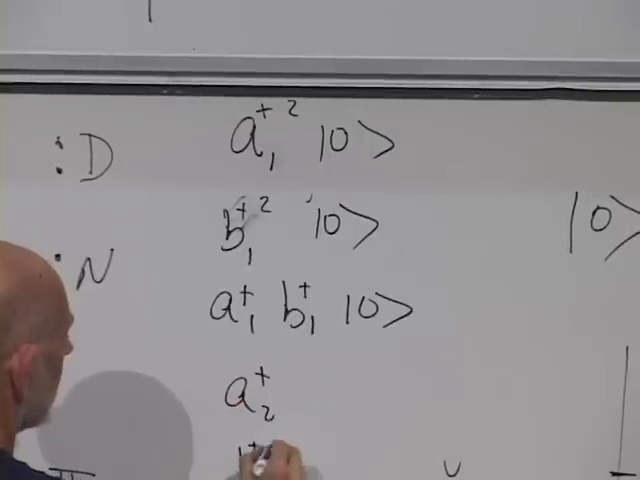
\includegraphics[width=0.76\textwidth]{lecture_02_figure_22.png}
  \caption{在听众质疑之后重新清点五个第二能级态：两个双激发、一个混合激发，以及两个第二谐波激发。}
  \lectureframe{01:44:00}
  \label{fig:l02-levels-board}
\end{figure}

\begin{figure}[H]
  \centering
  \begin{adjustbox}{max width=\linewidth}
  \begin{tikzpicture}[>=Latex,thick]
    \draw[->] (0,0) -- (0,5.1) node[above] {\(\Delta E_{\rm int}\)};
    \draw[blue!70!black] (-0.65,0.55) -- (0.65,0.55);
    \node[right] at (0.85,0.55) {\(\ket{0}\) \quad multiplicity \(1\)};
    \draw[blue!70!black] (-0.65,2.15) -- (0.65,2.15);
    \node[right] at (0.85,2.15)
      {\(a_1^\dagger\ket{0},\ b_1^\dagger\ket{0}\)
      \quad multiplicity \(2\)};
    \draw[blue!70!black] (-0.65,3.75) -- (0.65,3.75);
    \node[right,text width=8.6cm] at (0.85,3.75)
      {\((a_1^\dagger)^2\ket{0},
      a_1^\dagger b_1^\dagger\ket{0},
      (b_1^\dagger)^2\ket{0},
      a_2^\dagger\ket{0},\ b_2^\dagger\ket{0}\)
      \quad multiplicity \(5\)};
    \node[left] at (-0.75,0.55) {\(0\)};
    \node[left] at (-0.75,2.15) {\(1\)};
    \node[left] at (-0.75,3.75) {\(2\)};
  \end{tikzpicture}
  \end{adjustbox}
  \caption{两个横向方向的开弦的前三个激发能级。}
\label{fig:l02-levels-redraw}
\end{figure}

\begin{classroomqa}
\audiencequestion{第二激发态有四个还是五个态？\lecturetimestamp{01:43:04}}
\lecturerresponse{五个。将\(X_1\)激发两次、将\(Y_1\)激发两次，以及将二者各激发一次，给出三个态。将\(X_2\)激发一次或将\(Y_2\)激发一次，又给出两个态。所提议的练习是数出接下来的两个能级。}
\end{classroomqa}

本质性的结论已经显现。相邻能级之间由有限间隙分隔，且每个能级都具有有限的重数。因此，按照将其与咖啡、气体或普通小提琴弦区分开来的谱判据，量子化弦是类粒子的。稍后我们将确定哪些态在物理上是可接受的，以及哪些病态必须被去除。

\section{为什么开弦相互作用会产生闭弦}

开弦有两个端点。它的基本相互作用使弦连接和分裂。在强子图像中，可以想象一端是夸克、另一端是反夸克；它们的湮灭使两段弦连接起来。稍后所关注的基本弦不必带有那种字面意义上的强子端点解释，但局域的连接规则仍然成立。

现在让一根开弦涨落，直到它自己的两个端点彼此接近。局域地看，一个端点无法知道另一个端点属于同一根弦而不是另一根弦。如果端点终究可以连接，那么它们就可以在这里连接，从而产生一个闭合的圈。

\begin{figure}[H]
  \centering
  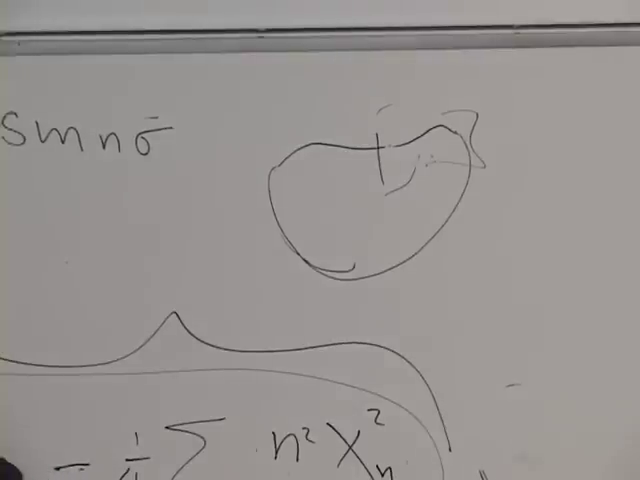
\includegraphics[width=0.70\textwidth]{lecture_02_figure_23.png}
  \caption{开弦涨落直至其两个端点相遇并形成一个闭合圈的板书示意图。}
  \lectureframe{01:47:00}
  \label{fig:l02-closed-board}
\end{figure}

\begin{figure}[H]
  \centering
  \begin{adjustbox}{max width=\linewidth}
  \begin{tikzpicture}[>=Latex,thick]
    \begin{scope}
      \draw[blue!70!black]
        (0,0) .. controls (0.8,1.2) and (1.7,-1.0) .. (2.6,0.45)
        .. controls (3.4,1.55) and (4.0,0.3) .. (4.7,0.85);
      \fill (0,0) circle (0.09);
      \fill (4.7,0.85) circle (0.09);
      \node at (2.35,-1.25) {open string fluctuation};
    \end{scope}
    \draw[->,line width=1pt] (5.25,0.3) -- (6.65,0.3)
      node[midway,above] {join};
    \begin{scope}[xshift=8.1cm]
      \draw[orange!85!black]
        (0,0) .. controls (0.3,1.5) and (2.5,1.8) .. (3.1,0.3)
        .. controls (3.5,-1.1) and (0.7,-1.5) .. (0,0);
      \node at (1.55,-1.85) {closed string};
    \end{scope}
  \end{tikzpicture}
  \end{adjustbox}
  \caption{一旦允许端点连接，开弦就可以自身闭合。}
  \label{fig:l02-closed-redraw}
\end{figure}

因此，一个理论可以包含闭弦而不包含开弦，但一个带有开弦的相互作用理论无法自洽地避免闭弦。这种不对称性就是重要的预言。谱的对应关系将在稍后展开，但目标已经显现：无质量的开弦态常常提供诸如光子之类的规范粒子，而闭弦谱则包含一个无质量的自旋二态，即引力子。一旦弦理论是相互作用的，闭弦、因而引力，就不是可有可无的装饰。
